\section{Location Discretization and Feature Computation} \label{sec:discretization_and_featurization}

\paragraph{Location Discretization}
The fewer possible discrete locations $l_i = (x,y,s)$, with $i = 1 \dots N$, we consider, the smaller our state space and therefore the better our reinforcement learning solution for a given amount of computation.
Featurization also takes less time as tolerable coarseness increases.
At the same time, we lose power to match ground truth detections.

There are three factors in the discretization process: the stride of the center point of the window $(x,y)$, and the number of octaves and scales per octave of $s$.

\note{todo: include a figure plotting oracle performance vs. decreasing coarseness of the image pyramid discretization.}

\paragraph{Coarse-to-Fine Evaluation}
The standard scale-invariant approach to detection with a template is to evaluate a template of fixed size over different scales of the image pyramid.
A recent report makes the observation that this approach using high-resolution, part-based models performs worse than scale-variant detection that degrades to using low-resolution, rigid models for detection at small scales of the image~\cite{Park2010}.
They demonstrate state-of-the-art results on a pedestrian detection benchmark.
The authors also note that context is most helpful for small-object detections.

\begin{figure}[h!]
  \caption{Illustration of the idea of using low-res models to approximate the output of high-res models, allowing us to only compute the image pyramid at small scales.}
  \centering
    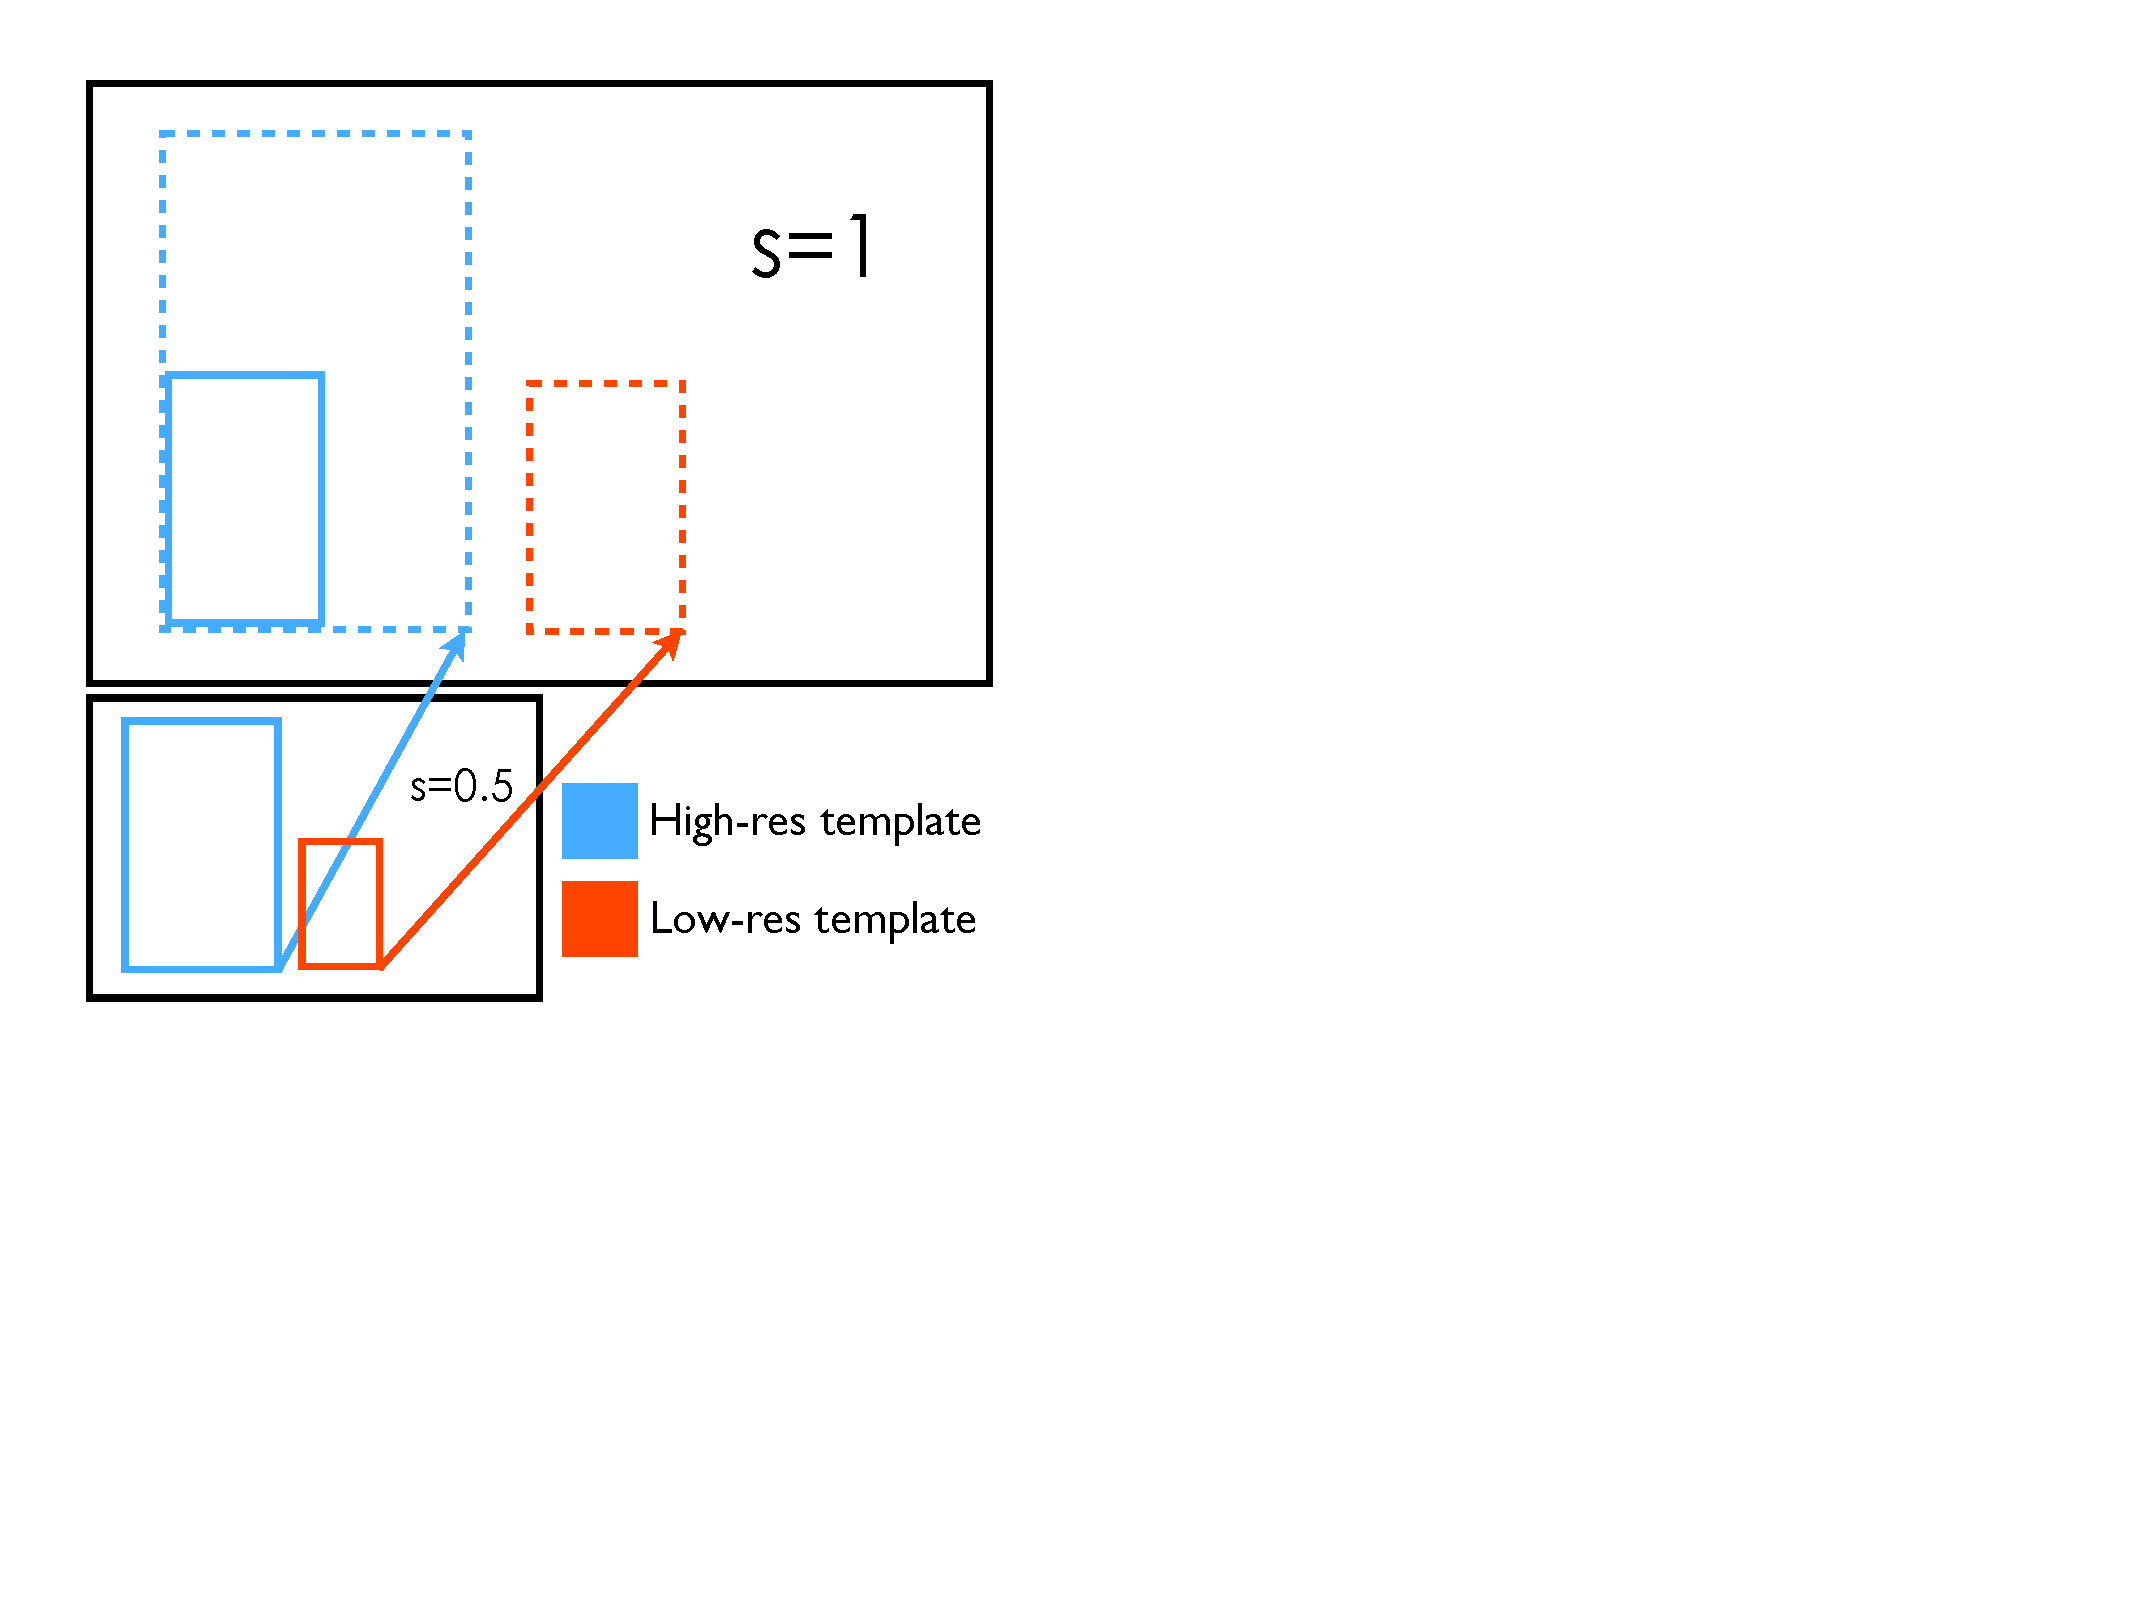
\includegraphics[width=0.7\textwidth]{../figures/multiscale.pdf}
  \label{fig:multiscale}
\end{figure}
We note also that a low-resolution model used at scale $s/2$ provides an approximation to the output of a high-resolution model at scale $s$, as illustrated in~\autoref{fig:multiscale}.
This may allow us to stagger feature computation, first computing just the small-scale part of the pyramid and running low-res models, and then computing the the large-scale part of the pyramid as time allows.

\paragraph{Feature Computation}
\note{todo: how can we include feature computation as part of the action space?}

\note{should look at Piotr Dollar's work on efficient HOG computation~\cite{Dollar2010}.}